  \section[OpenStack]{OpenStack : projet, logiciel et utilisation}

  \subsection[OpenStack]{Présentation du projet et du logiciel}

  \begin{frame}
    \frametitle{Vue haut niveau}
    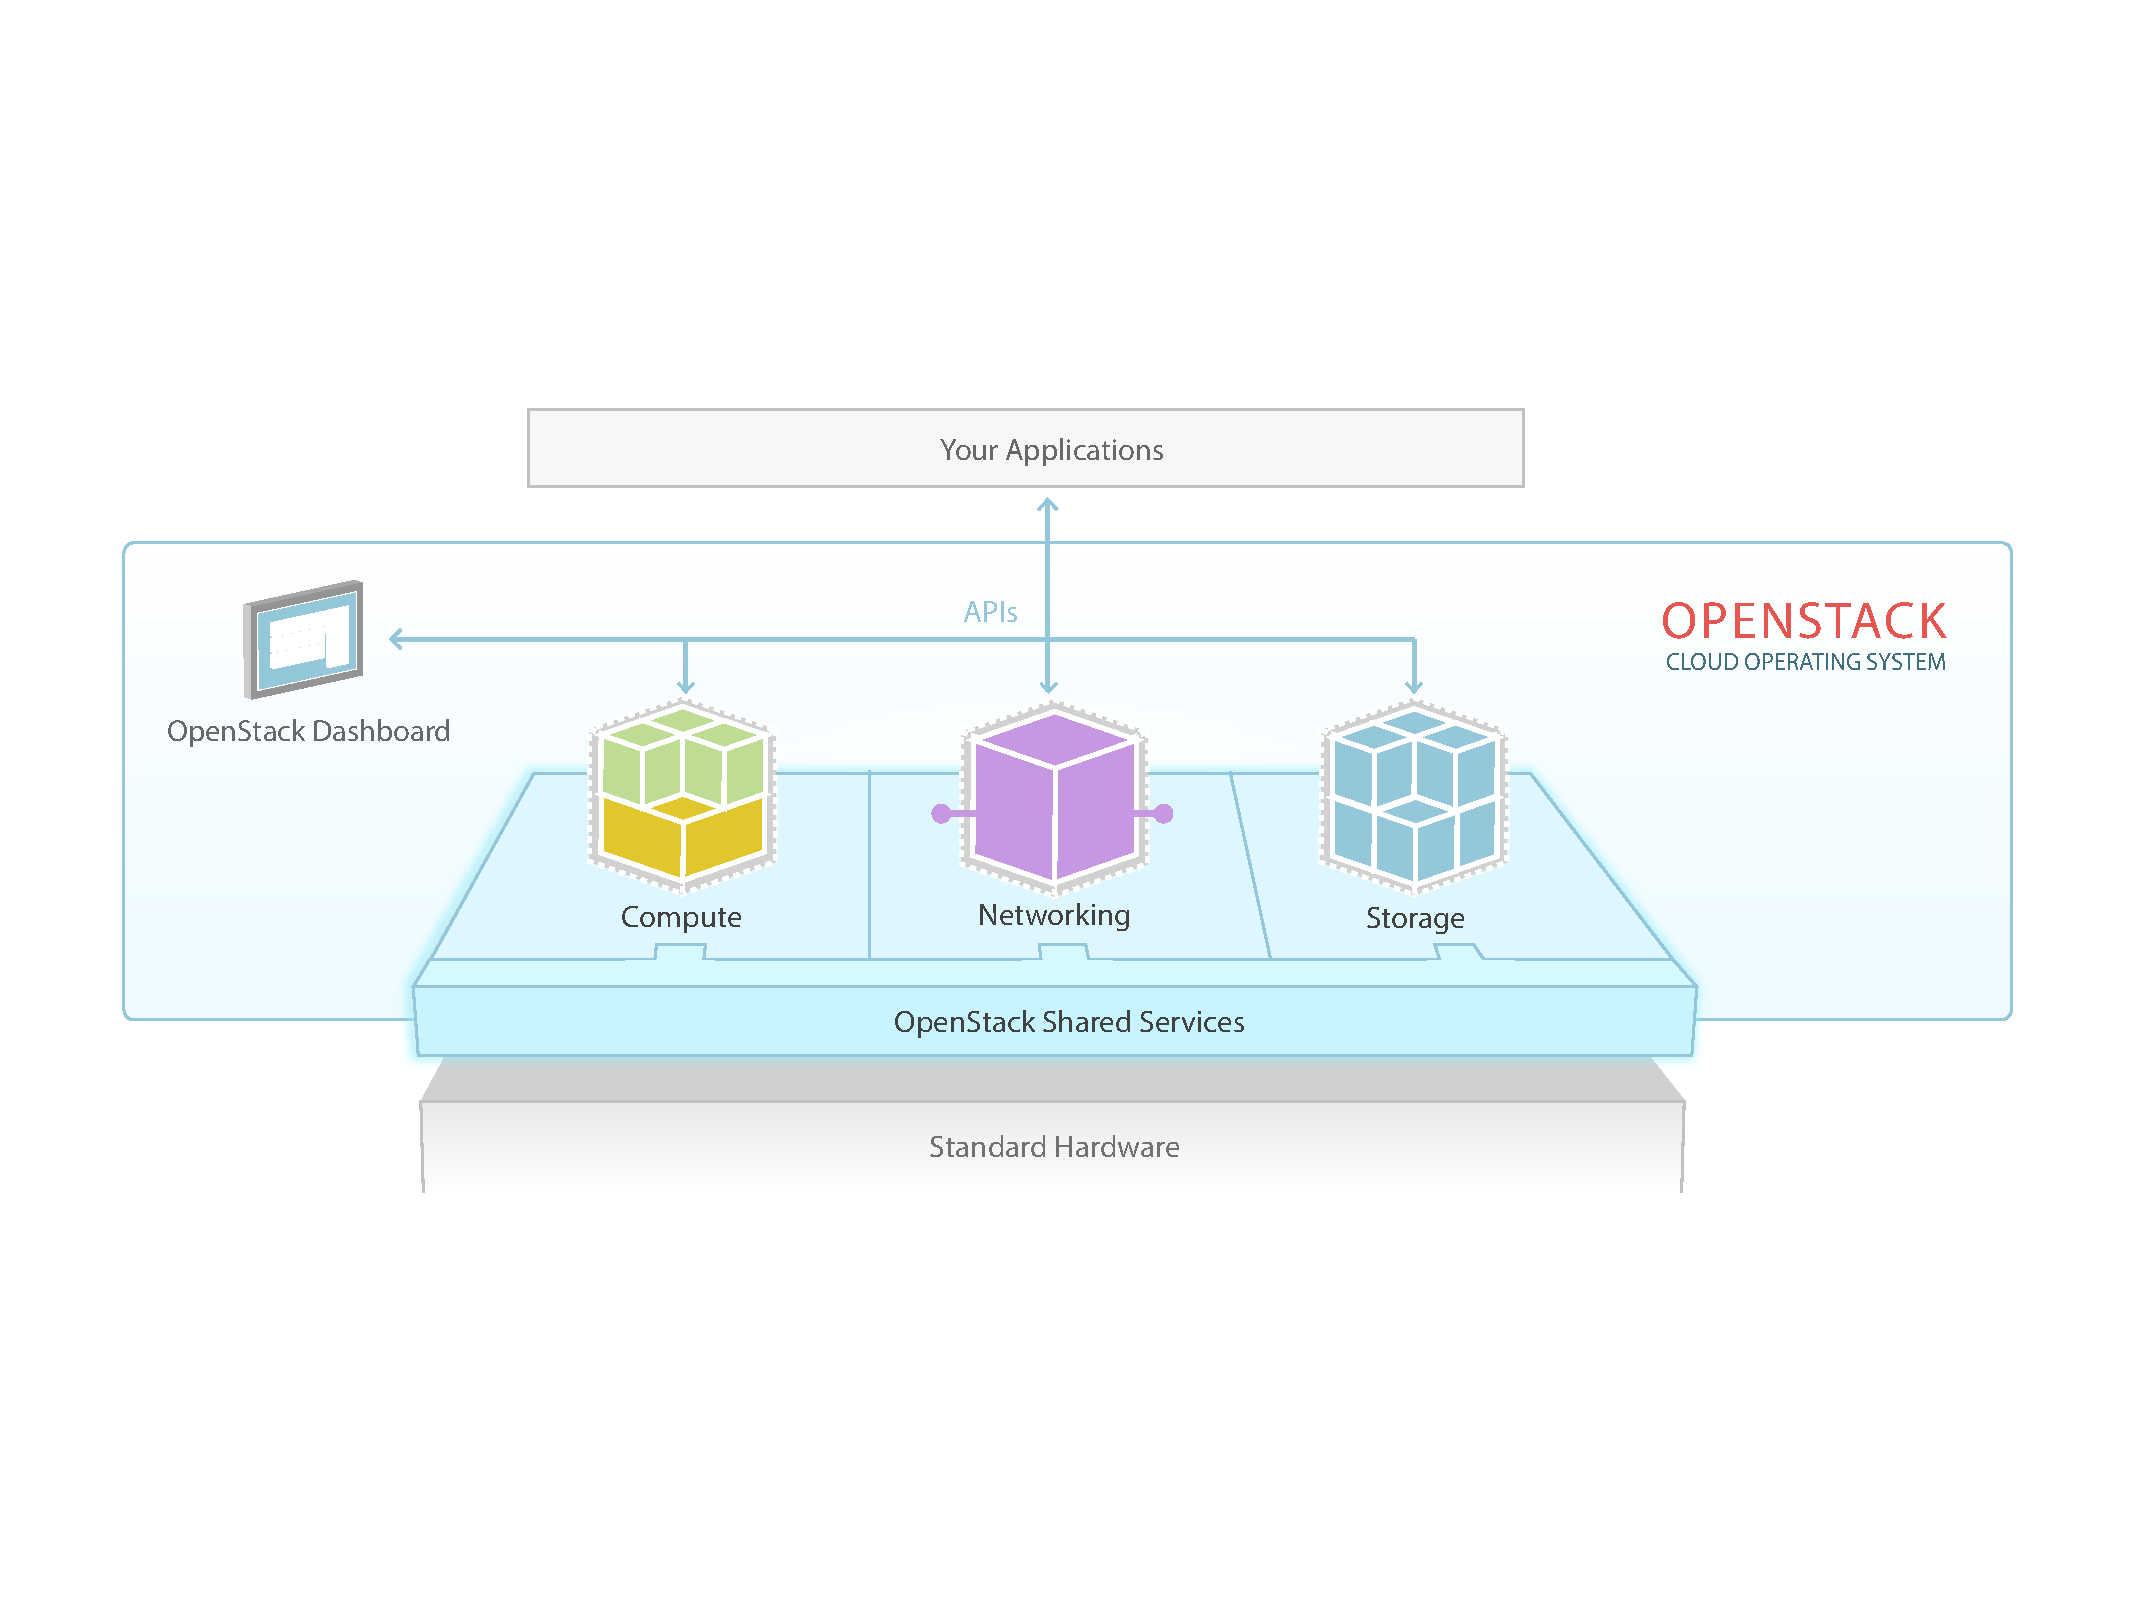
\includegraphics[width=\textwidth]{images/openstack-software-diagram.pdf}
  \end{frame}

  \begin{frame}
    \frametitle{Historique}
    \begin{itemize}
      \item Démarrage en 2010
      \item Objectif : le Cloud Operating System libre
      \item Fusion de deux projets de Rackspace (Storage) et de la NASA (Compute)
      \item Développé en Python et distribué sous licence Apache 2.0\pause
      \item Les releases jusqu'à aujourd'hui :
      \begin{itemize}
        \item Austin (2010.1)
        \item Bexar (2011.1)
        \item Cactus (2011.2)
        \item Diablo (2011.3)
        \item Essex (2012.1)
        \item Folsom (2012.2)
        \item Grizzly (2013.1)
        \item Havana (2013.2)
        \item Icehouse (2014.1)
        \item \textbf{Juno (2014.2)}\pause
        \item Avril 2015 : Kilo
      \end{itemize}
    \end{itemize}
  \end{frame}

  \begin{frame}
    \frametitle{Quelques soutiens/contributeurs ...}
    \begin{itemize}
      \item \textcolor{blue}{Rackspace} et la NASA\pause
      \item \textcolor{blue}{Canonical}
      \item \textcolor{blue}{Red Hat}
      \item \textcolor{blue}{SUSE}\pause
      \item \textcolor{blue}{HP}
      \item \textcolor{blue}{IBM}
      \item \textcolor{cyan}{Dell}, \textcolor{cyan}{Intel}
      \item \textcolor{cyan}{Cisco}, \textcolor{cyan}{Juniper}\pause
      \item \textcolor{cyan}{NetApp}, VMWare\pause
      \item \textcolor{cyan}{Yahoo}, Bull\pause
      \item Mais aussi : \textcolor{cyan}{Mirantis}, eNovance (racheté par Red Hat), \textcolor{cyan}{DreamHost}, Hastexo, StackOps\pause
    \end{itemize}
    \url{http://www.openstack.org/foundation/companies/}
  \end{frame}

  \begin{frame}
    \frametitle{... et utilisateurs}
    \begin{itemize}
      \item Tous les contributeurs précédemment cités\pause
      \item En France : \textbf{Cloudwatt} et \textbf{Numergy}\pause
      \item Wikimedia
      \item CERN
      \item Paypal
      \item Comcast
      \item BMW\pause
      \item Etc. Sans compter les implémentations confidentielles
    \end{itemize}
    \url{http://www.openstack.org/user-stories/}
  \end{frame}

  \begin{frame}
    \frametitle{Les différents sous-projets}
    \begin{itemize}
        \item OpenStack Compute - Nova
        \item OpenStack (Object) Storage - Swift\pause
        \item OpenStack Block Storage - Cinder\pause
        \item OpenStack Networking - Neutron\pause
        \item OpenStack Image Service - Glance\pause
        \item OpenStack Identity Service - Keystone\pause
        \item OpenStack Dashboard - Horizon\pause
        \item OpenStack Telemetry - Ceilometer\pause
        \item OpenStack Orchestration - Heat\pause
        \item OpenStack Database Service - Trove
    \end{itemize}
  \end{frame}

  \begin{frame}
    \frametitle{Les différents sous-projets (2)}
    \begin{itemize}
      \item Incubating et/ou intéressants
      \begin{itemize}
        \item Bare metal (Ironic)
        \item Queue service (Zaqar)
        \item Data processing (Sahara)
        \item DNS service (Designate)
        \item Shared File Systems (Manila)
        \item Key management (Barbican)
        \item PaaS (Solum)
      \end{itemize}\pause
      \item Autres
      \begin{itemize}
        \item Oslo
        \item rootwrap : wrapper pour les commandes root utilisé par les projets
        \item TripleO
        \item Tempest, Grenade
        \item Les clients (python-*client)
      \end{itemize}
    \end{itemize}
  \end{frame}

  \begin{frame}
    \frametitle{Cycle de vie des projets au sein d'OpenStack}
    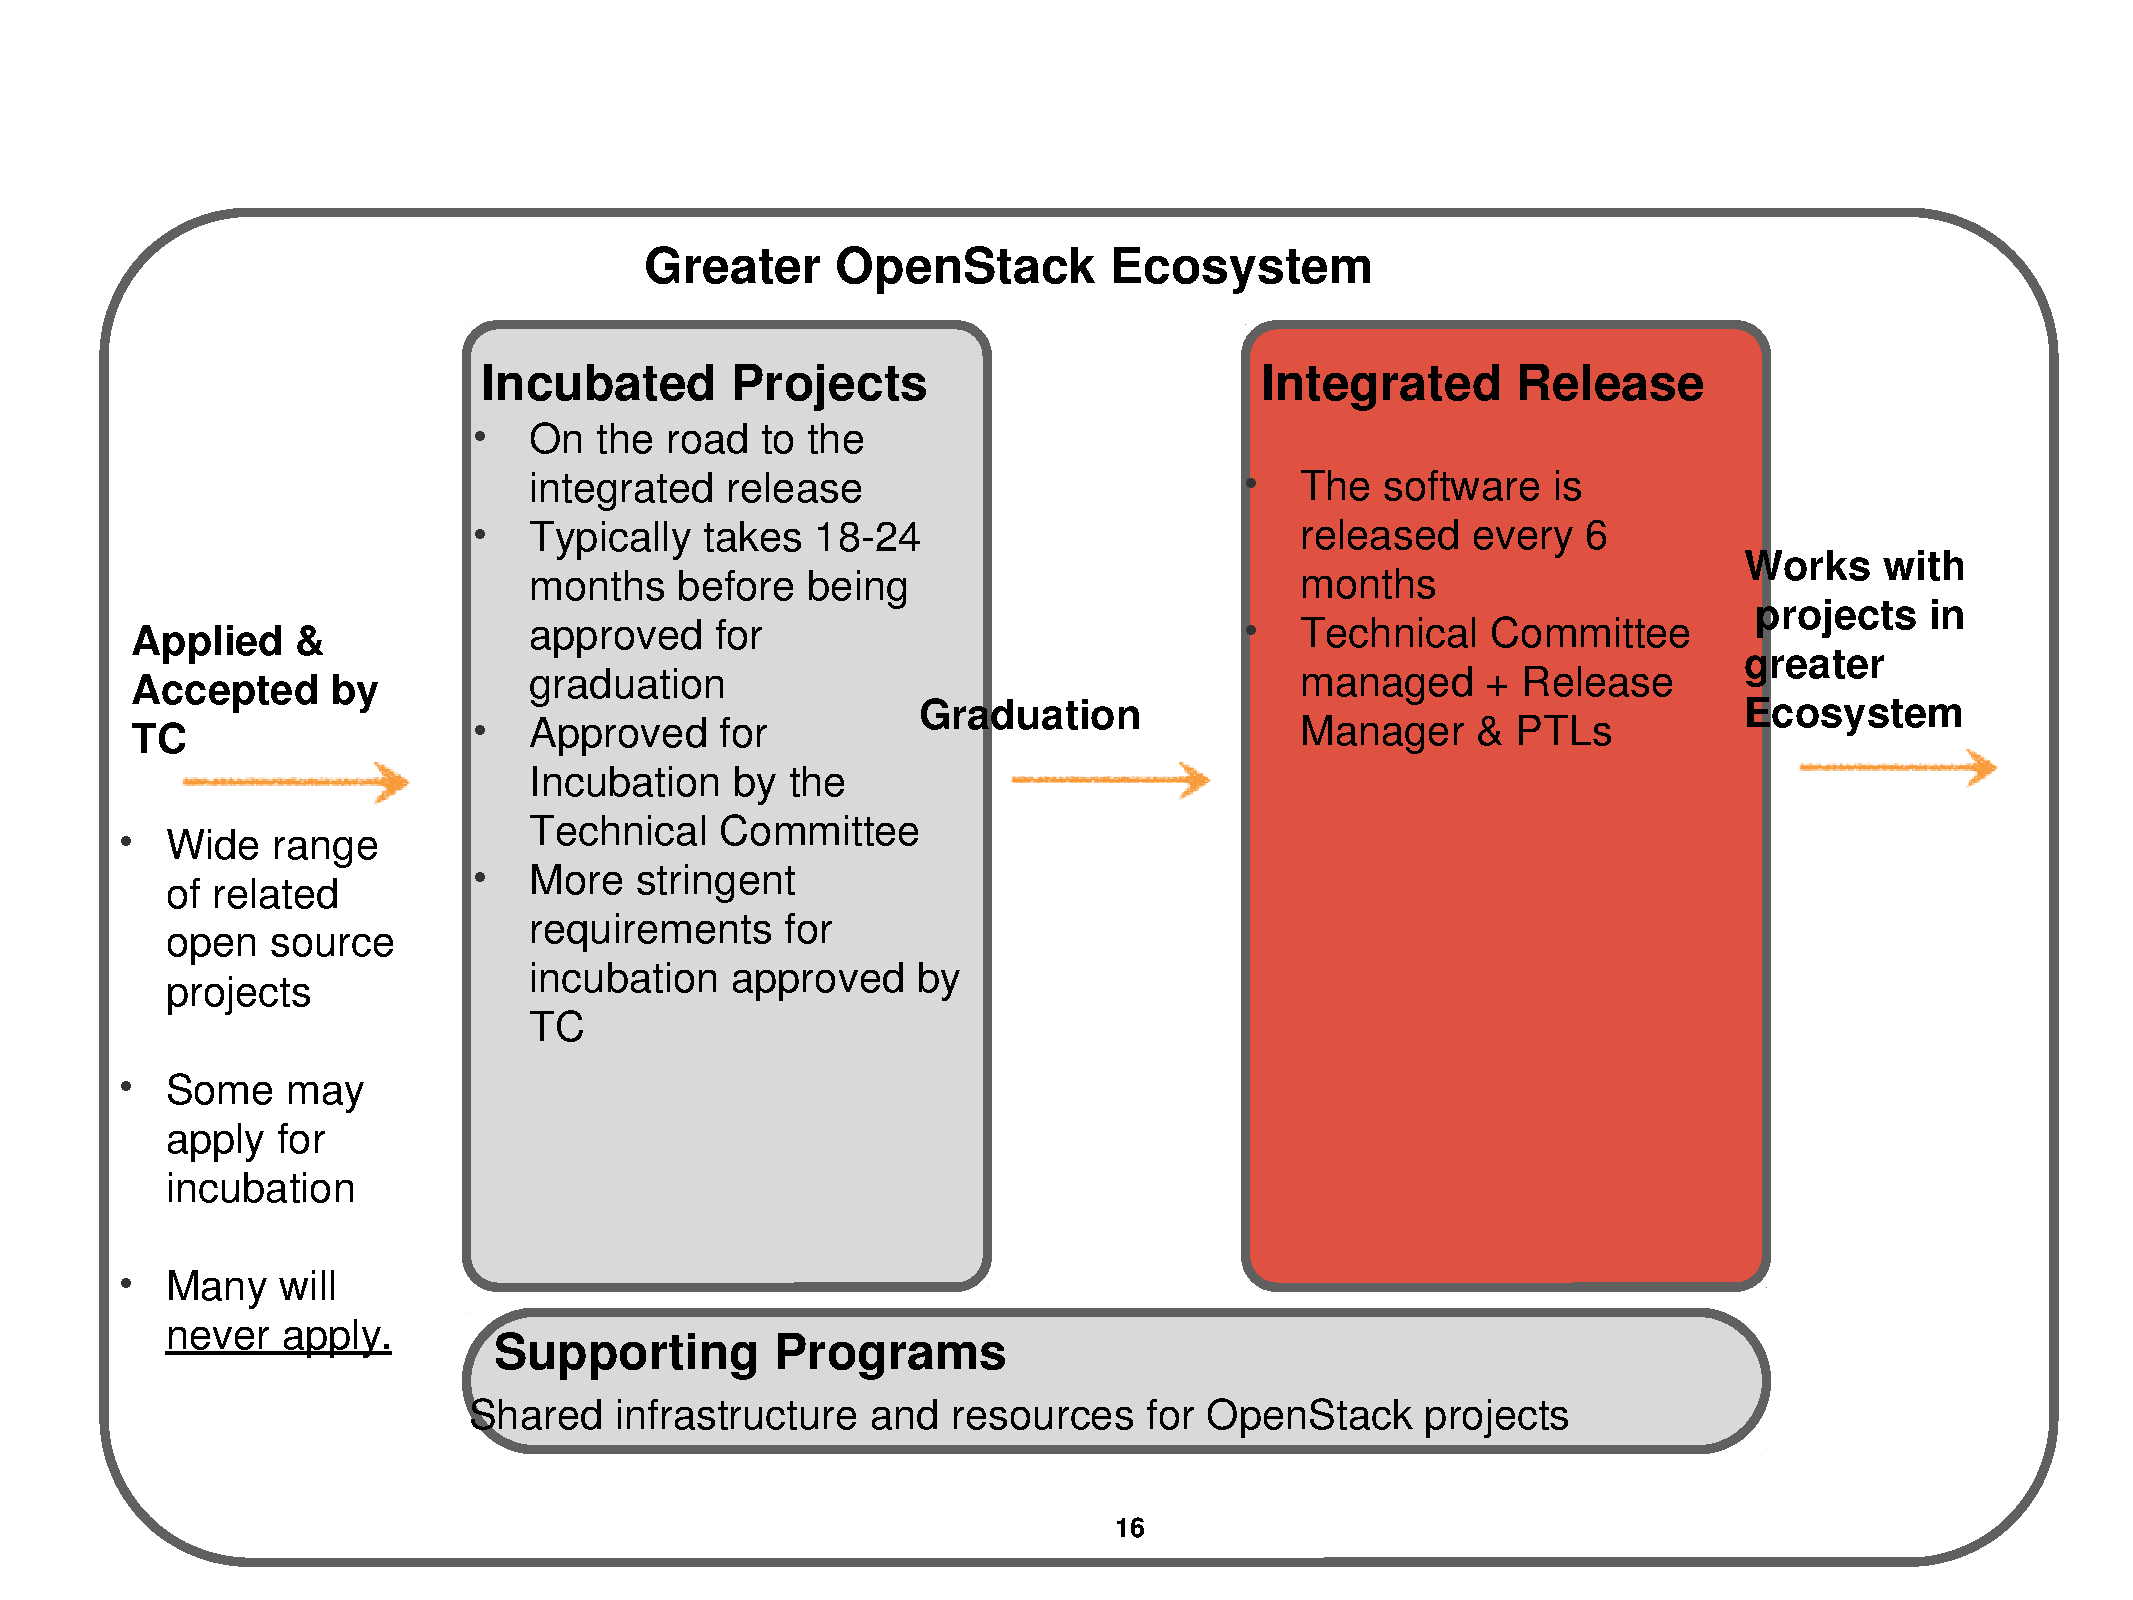
\includegraphics[width=\textwidth]{images/innovation1.pdf}
  \end{frame}

  \begin{frame}
    \frametitle{Les projets dans Icehouse}
    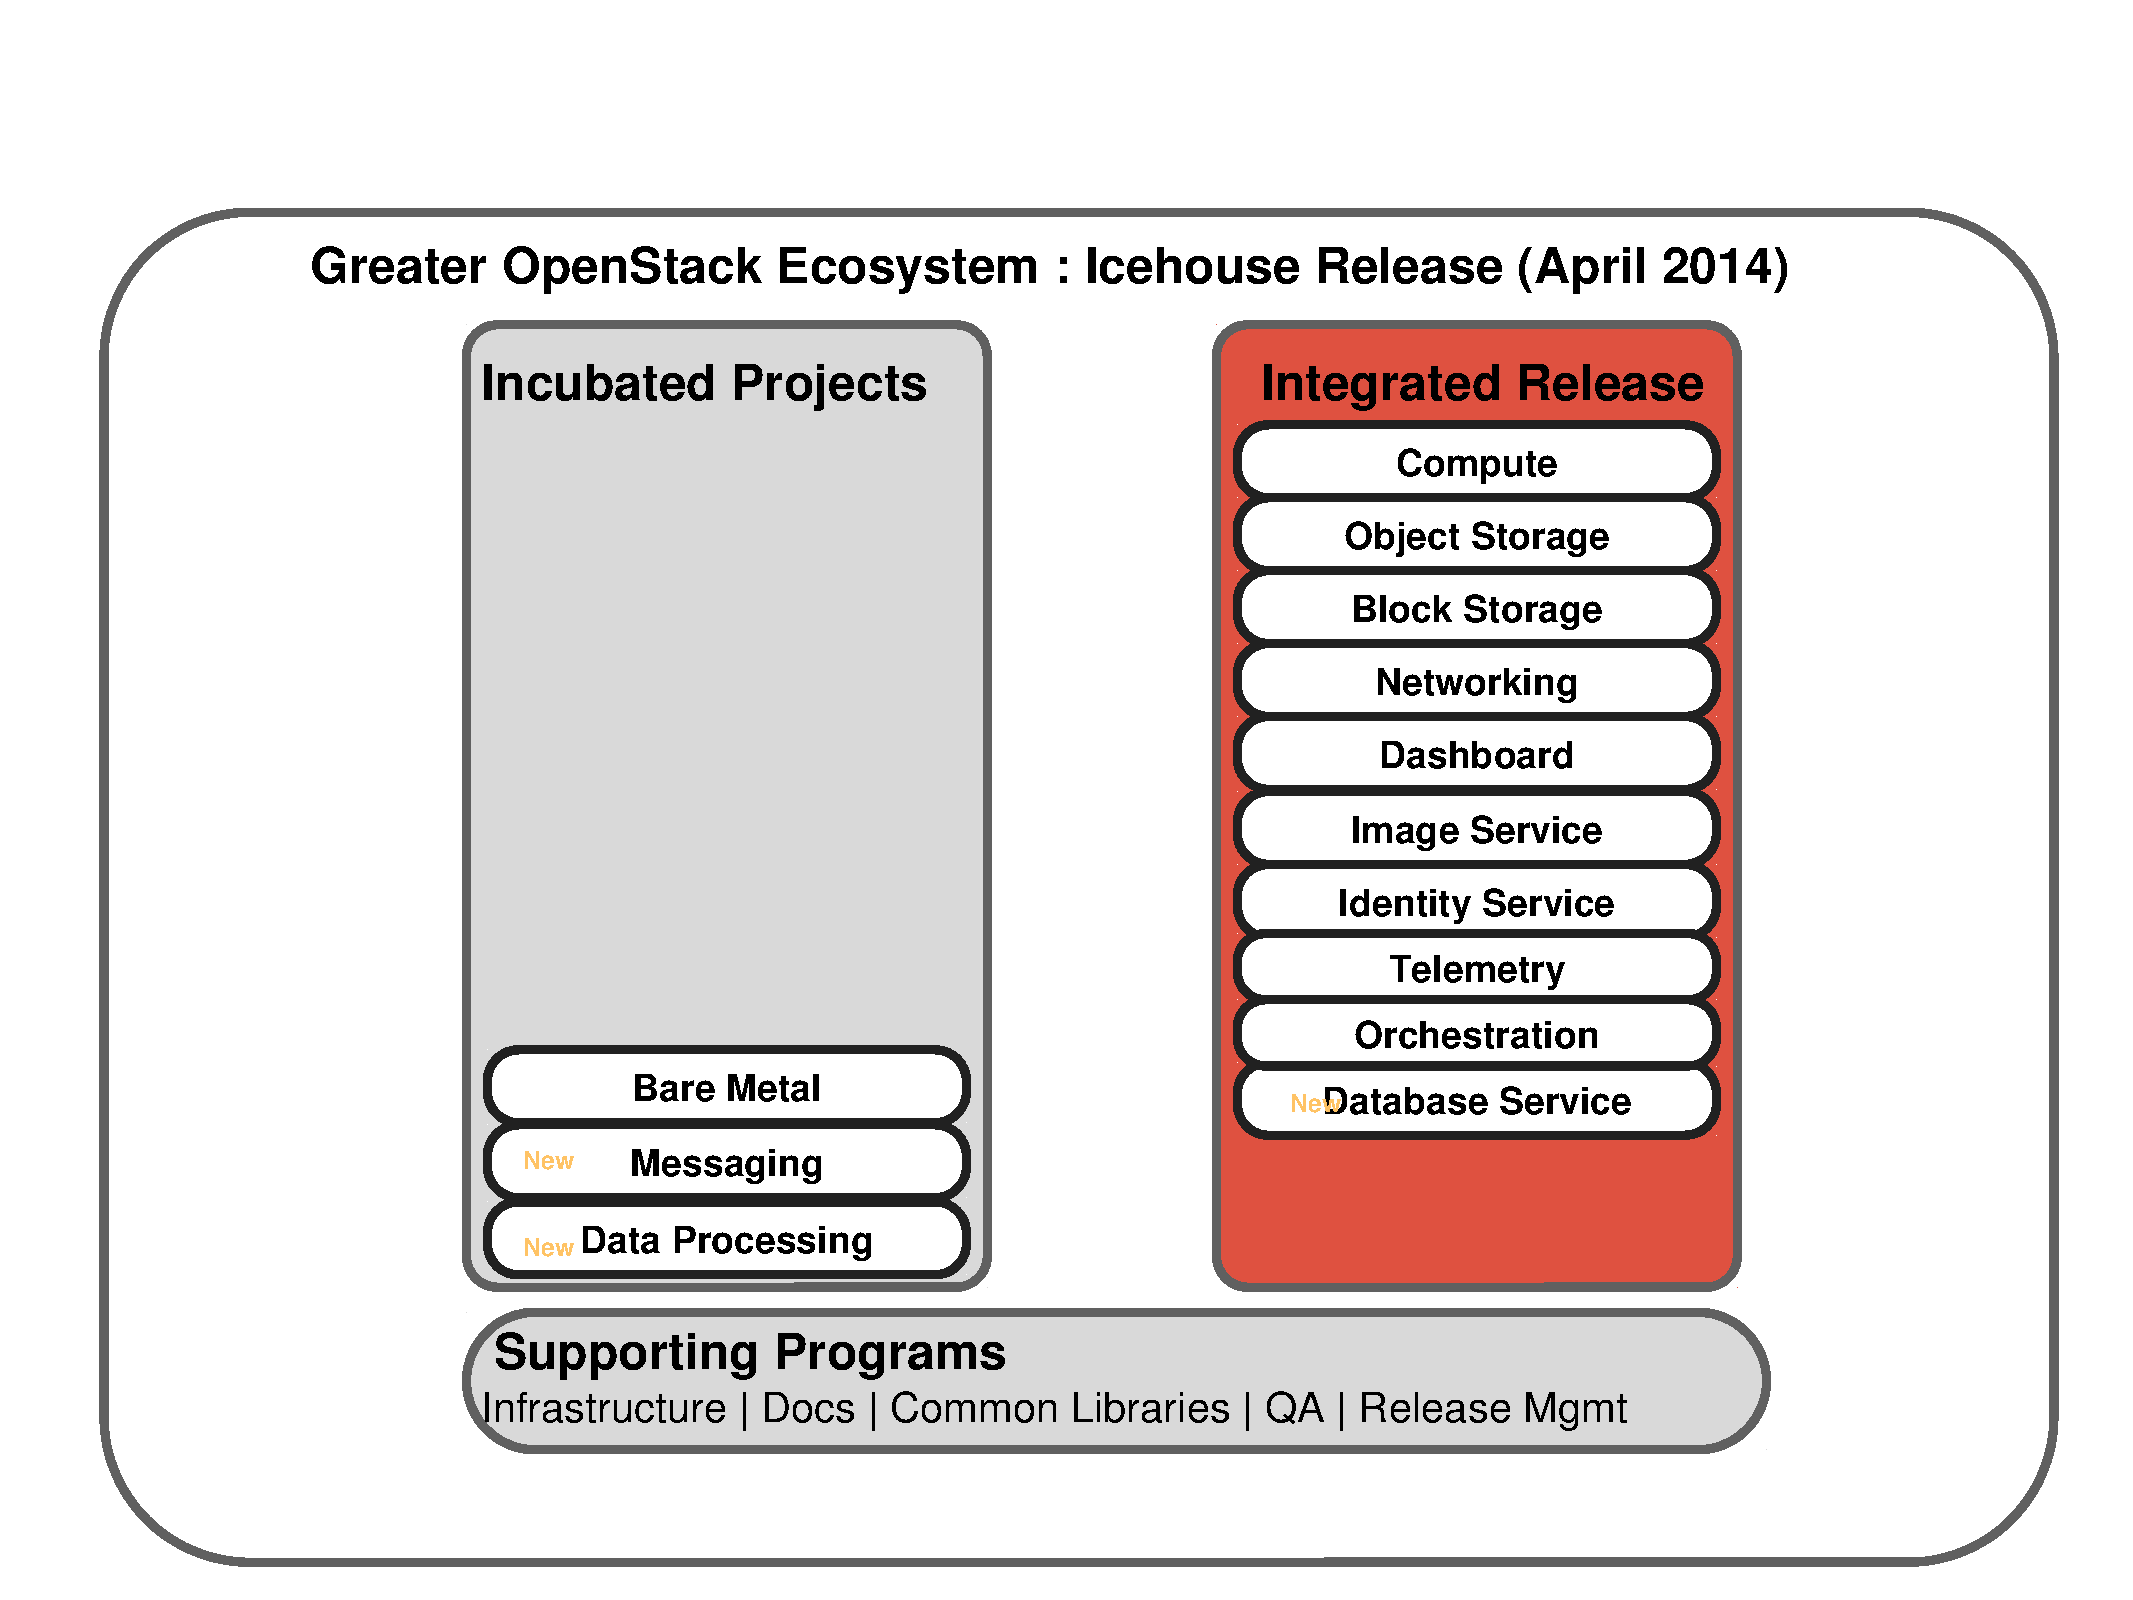
\includegraphics[width=\textwidth]{images/innovation2.pdf}
  \end{frame}

  \begin{frame}
    \frametitle{Le nouveau modèle "big tent"}
    \begin{itemize}
      \item Évolutions toujours en discussion
      \item Objectif : résoudre les limitations du modèle incubation/intégré
      \item Inclusion {a priori} de l'ensemble de l'écosystème OpenStack
      \item \textit{Programs} $\rightarrow$ \textit{Project Teams}
      \item Disparation des statuts en incubation et intégré
      \item Utilisation de tags factuels et objectifs
    \end{itemize}
  \end{frame}

  \begin{frame}
    \frametitle{Traduction}
    \begin{itemize}
      \item La question de la traduction est dorénavant prise en compte
      \item Seules certaines parties sont traduites, comme Horizon
      \item La traduction française est aujourd'hui une des plus avancées
      \item Utilisation de la plateforme Transifex
    \end{itemize}
  \end{frame}

  \begin{frame}
    \frametitle{Développement du projet : les principes}
    \begin{itemize}
      \item Open Source
      \item Open Design
      \item Open Development
      \item Open Community
    \end{itemize}
  \end{frame}

  \begin{frame}
    \frametitle{Développement du projet : en détails}
    \begin{itemize}
      \item Ouvert à tous (individuels et entreprises)\pause
      \item Cycle de développement de 6 mois débuté par un (design) summit\pause
      \item Outils : Launchpad $\rightarrow$ Storyboard (blueprints, bugs) + Git + GitHub (code)\pause
      \item Sur chaque patch proposé :
      \begin{itemize}
        \item Revue de code (peer review) : Gerrit, \url{https://review.openstack.org}
        \item Intégration continue (continous integration) : Jenkins, Zuul, etc., \url{http://zuul.openstack.org/}
      \end{itemize}\pause
      \item Développement hyper actif : 17000 commits dans Icehouse (+25\%)\pause
      \item Fin 2012, création d'une entité indépendante de gouvernance : la fondation OpenStack
    \end{itemize}
  \end{frame}

  \begin{frame}
    \frametitle{La fondation OpenStack}
    \begin{itemize}
      \item Entité de gouvernance principale du projet
      \item Représentation juridique du projet
      \item Les membres du board sont issus des entreprises sponsors et élus par les membres individuels
      \item Tout le monde peut devenir membre individuel (gratuitement)
      \item La fondation supporte le projet par différents moyens :
      \begin{itemize}
        \item Événements : organisation (Summits) ou participation (OSCON, etc.)
        \item Infrastructure de développement (serveurs)
        \item Ressources humaines : marketing, release manager, quelques développeurs (principalement sur l'infrastructure)
      \end{itemize}
      \item 850 organisations à travers le monde
      \item 9500 membres individuels dans 100 pays
    \end{itemize}
  \end{frame}

  \begin{frame}
    \frametitle{La fondation OpenStack}
      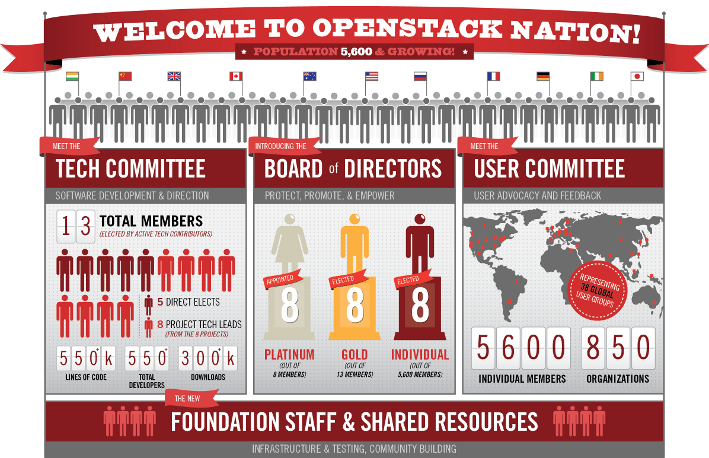
\includegraphics[width=\textwidth]{images/foundation.png}
  \end{frame}

  \begin{frame}
    \frametitle{Cycle de développement : 6 mois}
    \begin{itemize}
      \item Le planning est publié, exemple : \url{https://wiki.openstack.org/wiki/Kilo_Release_Schedule}
      \item Milestone releases
      \item Freezes : FeatureProposal, Feature, String
      \item RC releases
      \item Stable releases
      \item Ce modèle de cycle de développement a évolué depuis le début du projet
      \item Cas particulier de Swift
    \end{itemize}
  \end{frame}

  \begin{frame}
    \frametitle{Où trouver des informations sur le développement d'OpenStack}
    \begin{itemize}
      \item Principalement sur le wiki : \url{https://wiki.openstack.org}
      \item Les blueprints et bugs sur Launchpad/StoryBoard : \url{https://launchpad.net/openstack}, \url{https://storyboard.openstack.org}, \url{http://specs.openstack.org/}
      \item Les patchs proposés et leurs reviews sont sur Gerrit : \url{https://review.openstack.org}
      \item L'état de la CI (entre autres) : \url{http://status.openstack.org}
      \item Le code est disponible dans Git : \url{https://git.openstack.org}
      \item Les sources (tarballs) sont disponibles : \url{http://tarballs.openstack.org/}
    \end{itemize}
  \end{frame}

  \begin{frame}
    \frametitle{Qui contribue ?}
    \begin{itemize}
      \item \textit{Active Technical Contributor}
      \item ATC : personne ayant au moins une contribution récente dans un projet OpenStack reconnu
      \item Les ATC sont invités aux summits
      \item \textit{Core reviewer} : ATC ayant les droits pour valider les patchs dans un projet
      \item Stackalytics fournit des statistiques sur les contributions
    \end{itemize}
    \url{http://stackalytics.com/}
  \end{frame}

  \begin{frame}
    \frametitle{Stackforge}
    \begin{itemize}
      \item Forge pour les nouveaux projets en lien avec OpenStack
      \item Ils bénéficient de l'infrastructure du projet OpenStack, mais la séparation reste claire
      \item Les projets démarrent dans Stackforge et peuvent ensuite rejoindre le projet OpenStack
    \end{itemize}
  \end{frame}

  \begin{frame}
    \frametitle{OpenStack Summit}
    \begin{itemize}
      \item Aux USA jusqu'en 2013
      \item Aujourd'hui : alternance USA et Asie/Europe
      \item Quelques centaines au début à 4500 participants aujourd'hui
      \item En parallèle : conférence (utilisateurs, décideurs) et Design Summit (développeurs)
      \item Détermine le nom de la release : lieu/ville à proximité du Summit
      \item \textit{Upstream Training}
    \end{itemize}
  \end{frame}

  \begin{frame}
    \frametitle{Exemple du Summit d'avril 2013 à Portland}
    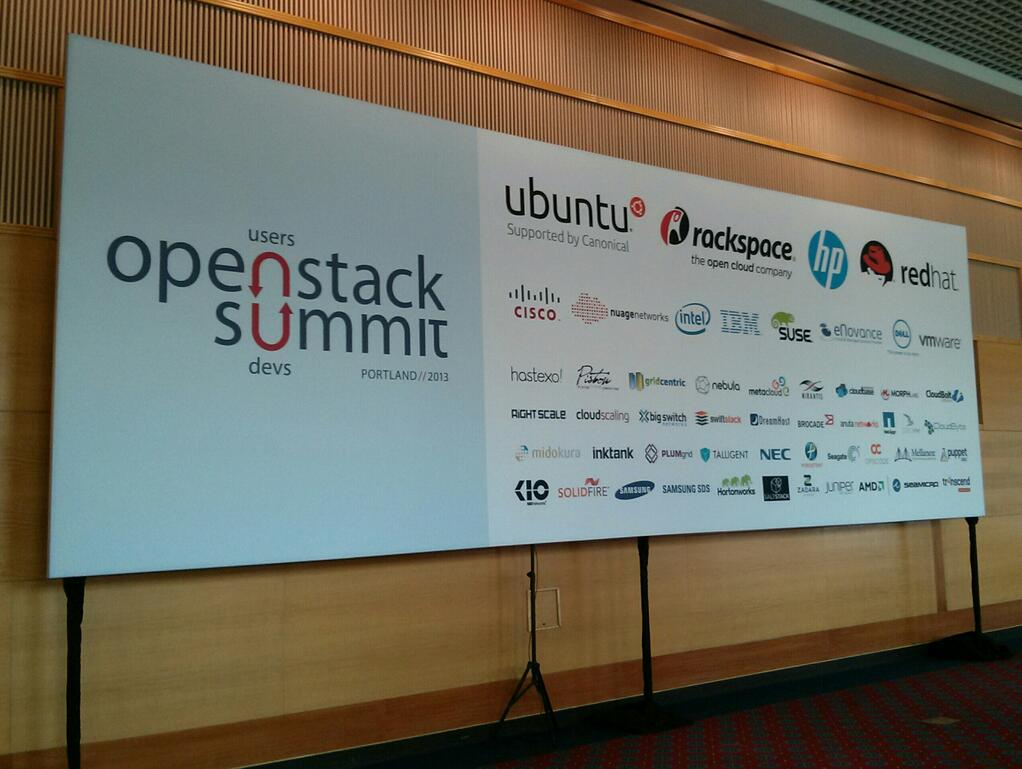
\includegraphics[width=\textwidth]{images/photo-summit.jpg}
  \end{frame}

  \begin{frame}
    \frametitle{Exemple du Summit de mai 2014 à Atlanta}
    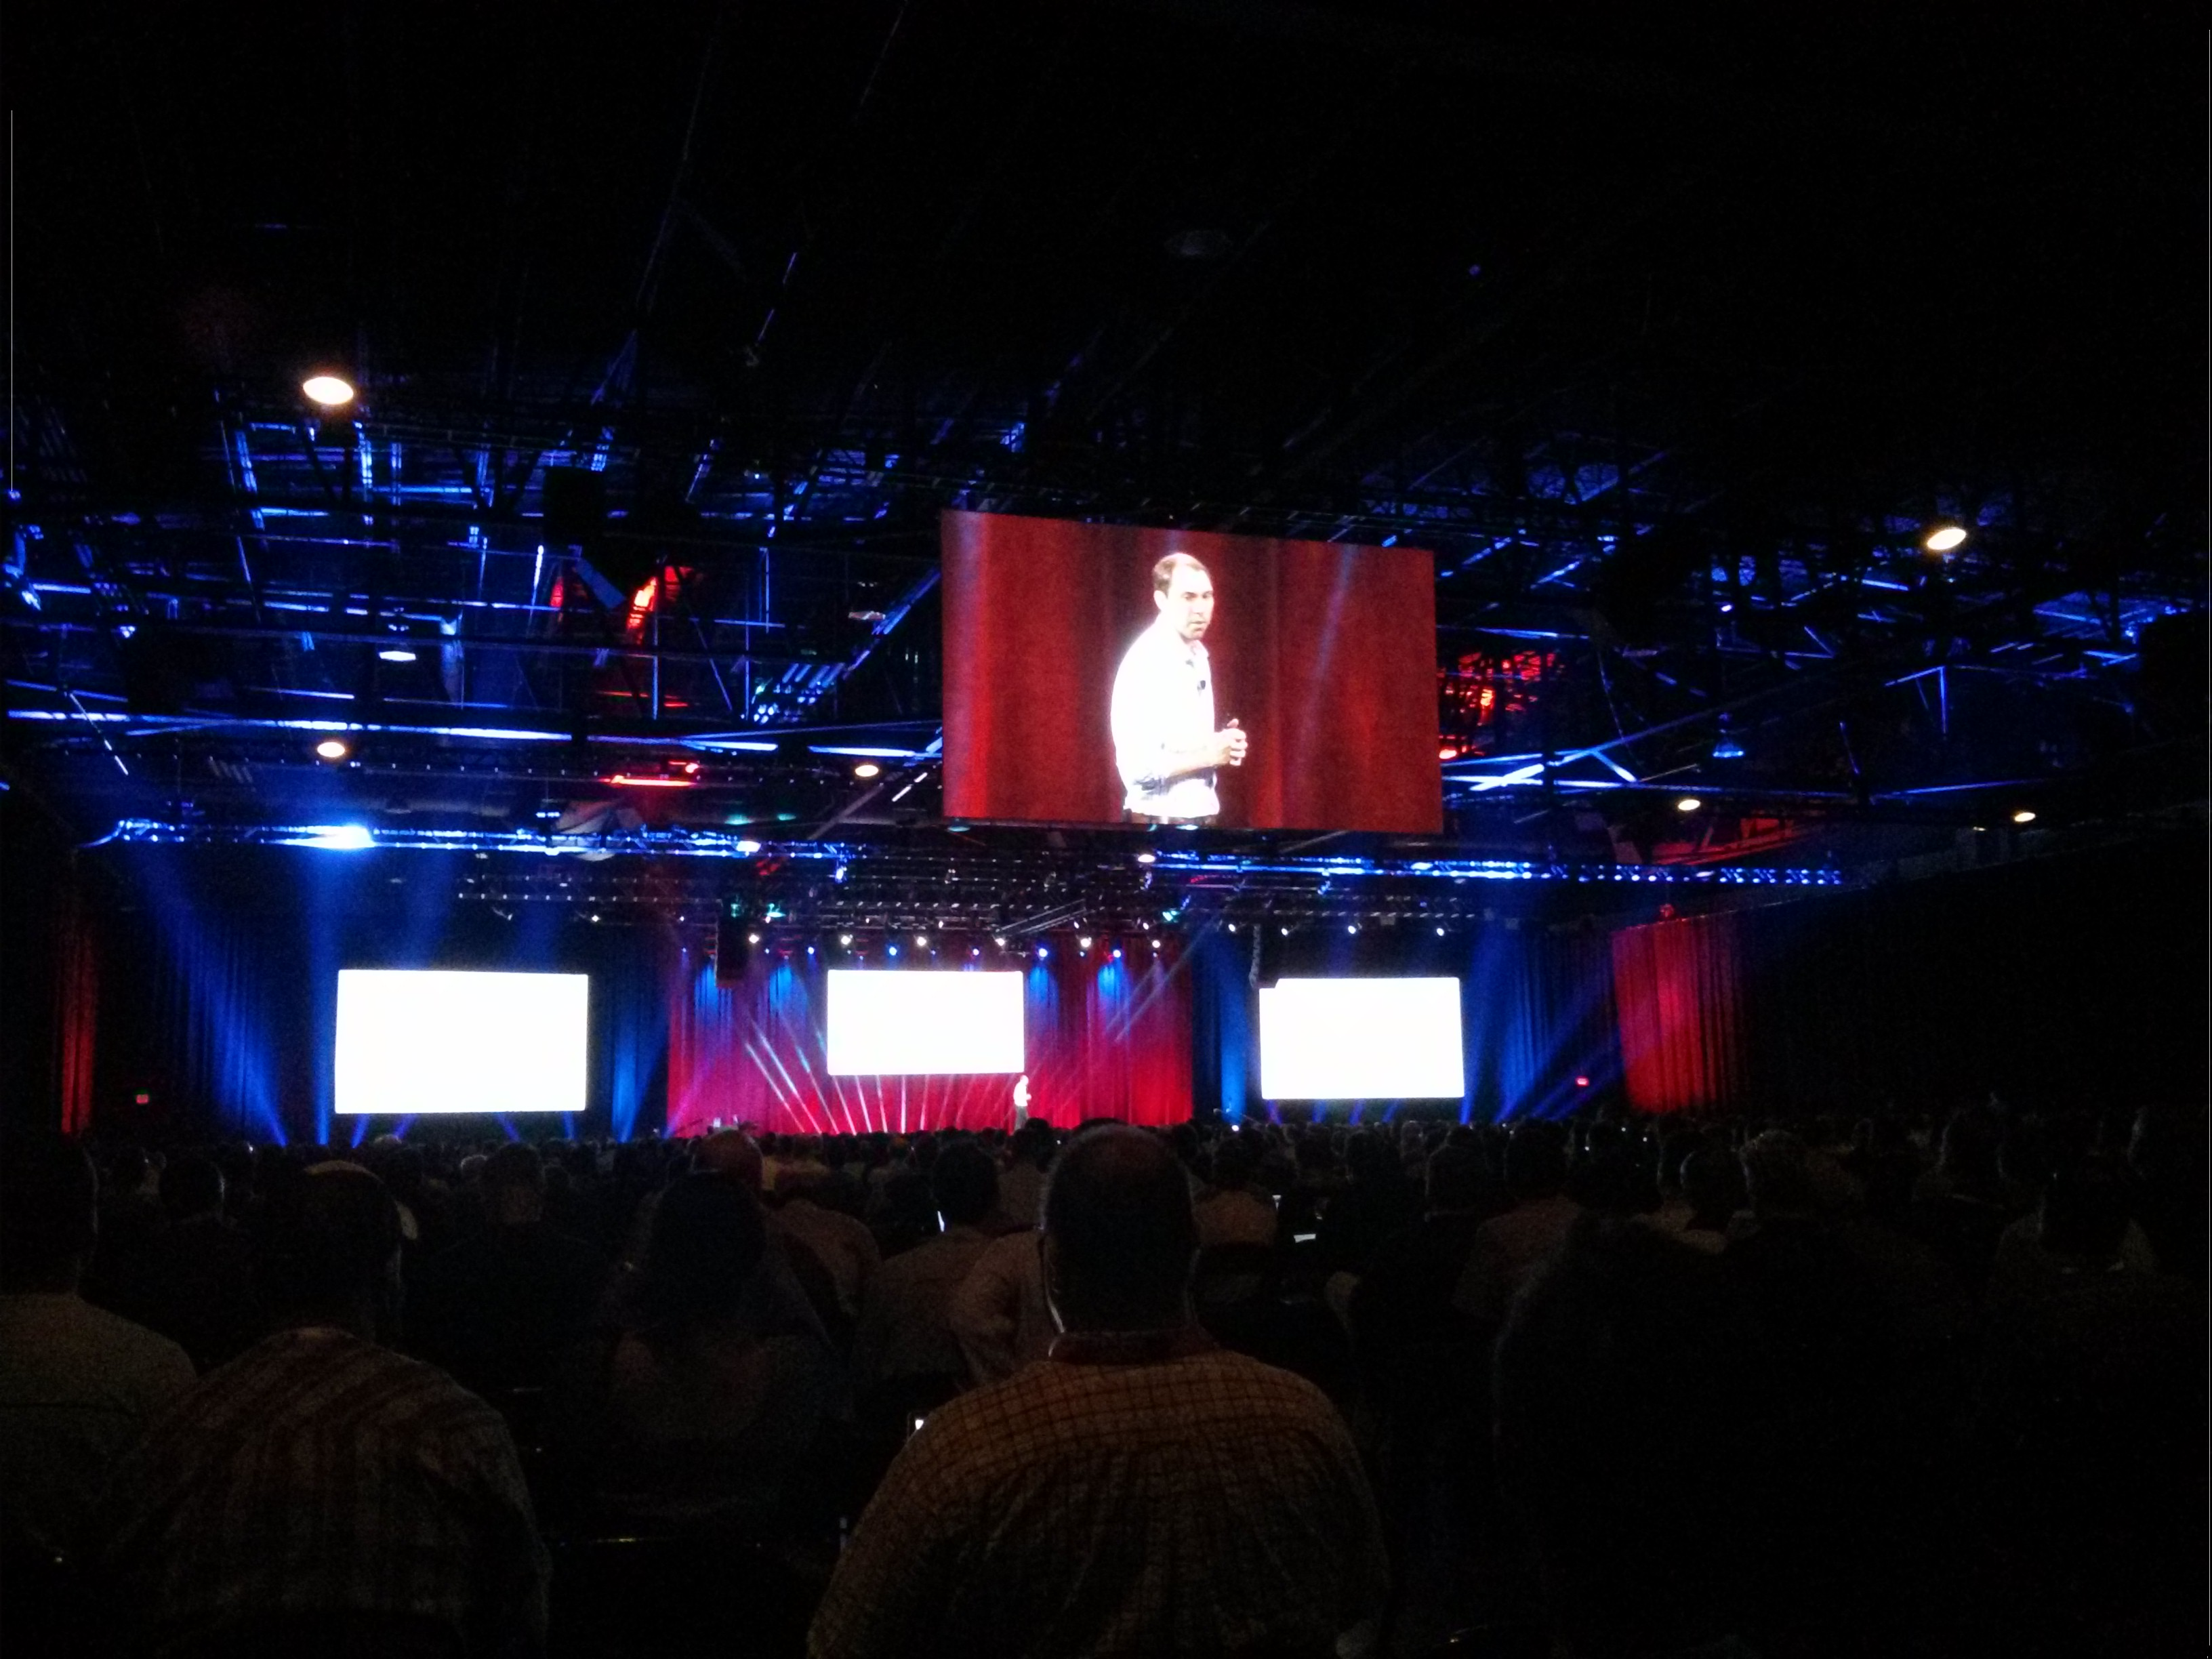
\includegraphics[width=\textwidth]{images/photo-summit1.jpg}
  \end{frame}

  \begin{frame}
    \frametitle{Exemple du Summit de mai 2014 à Atlanta}
    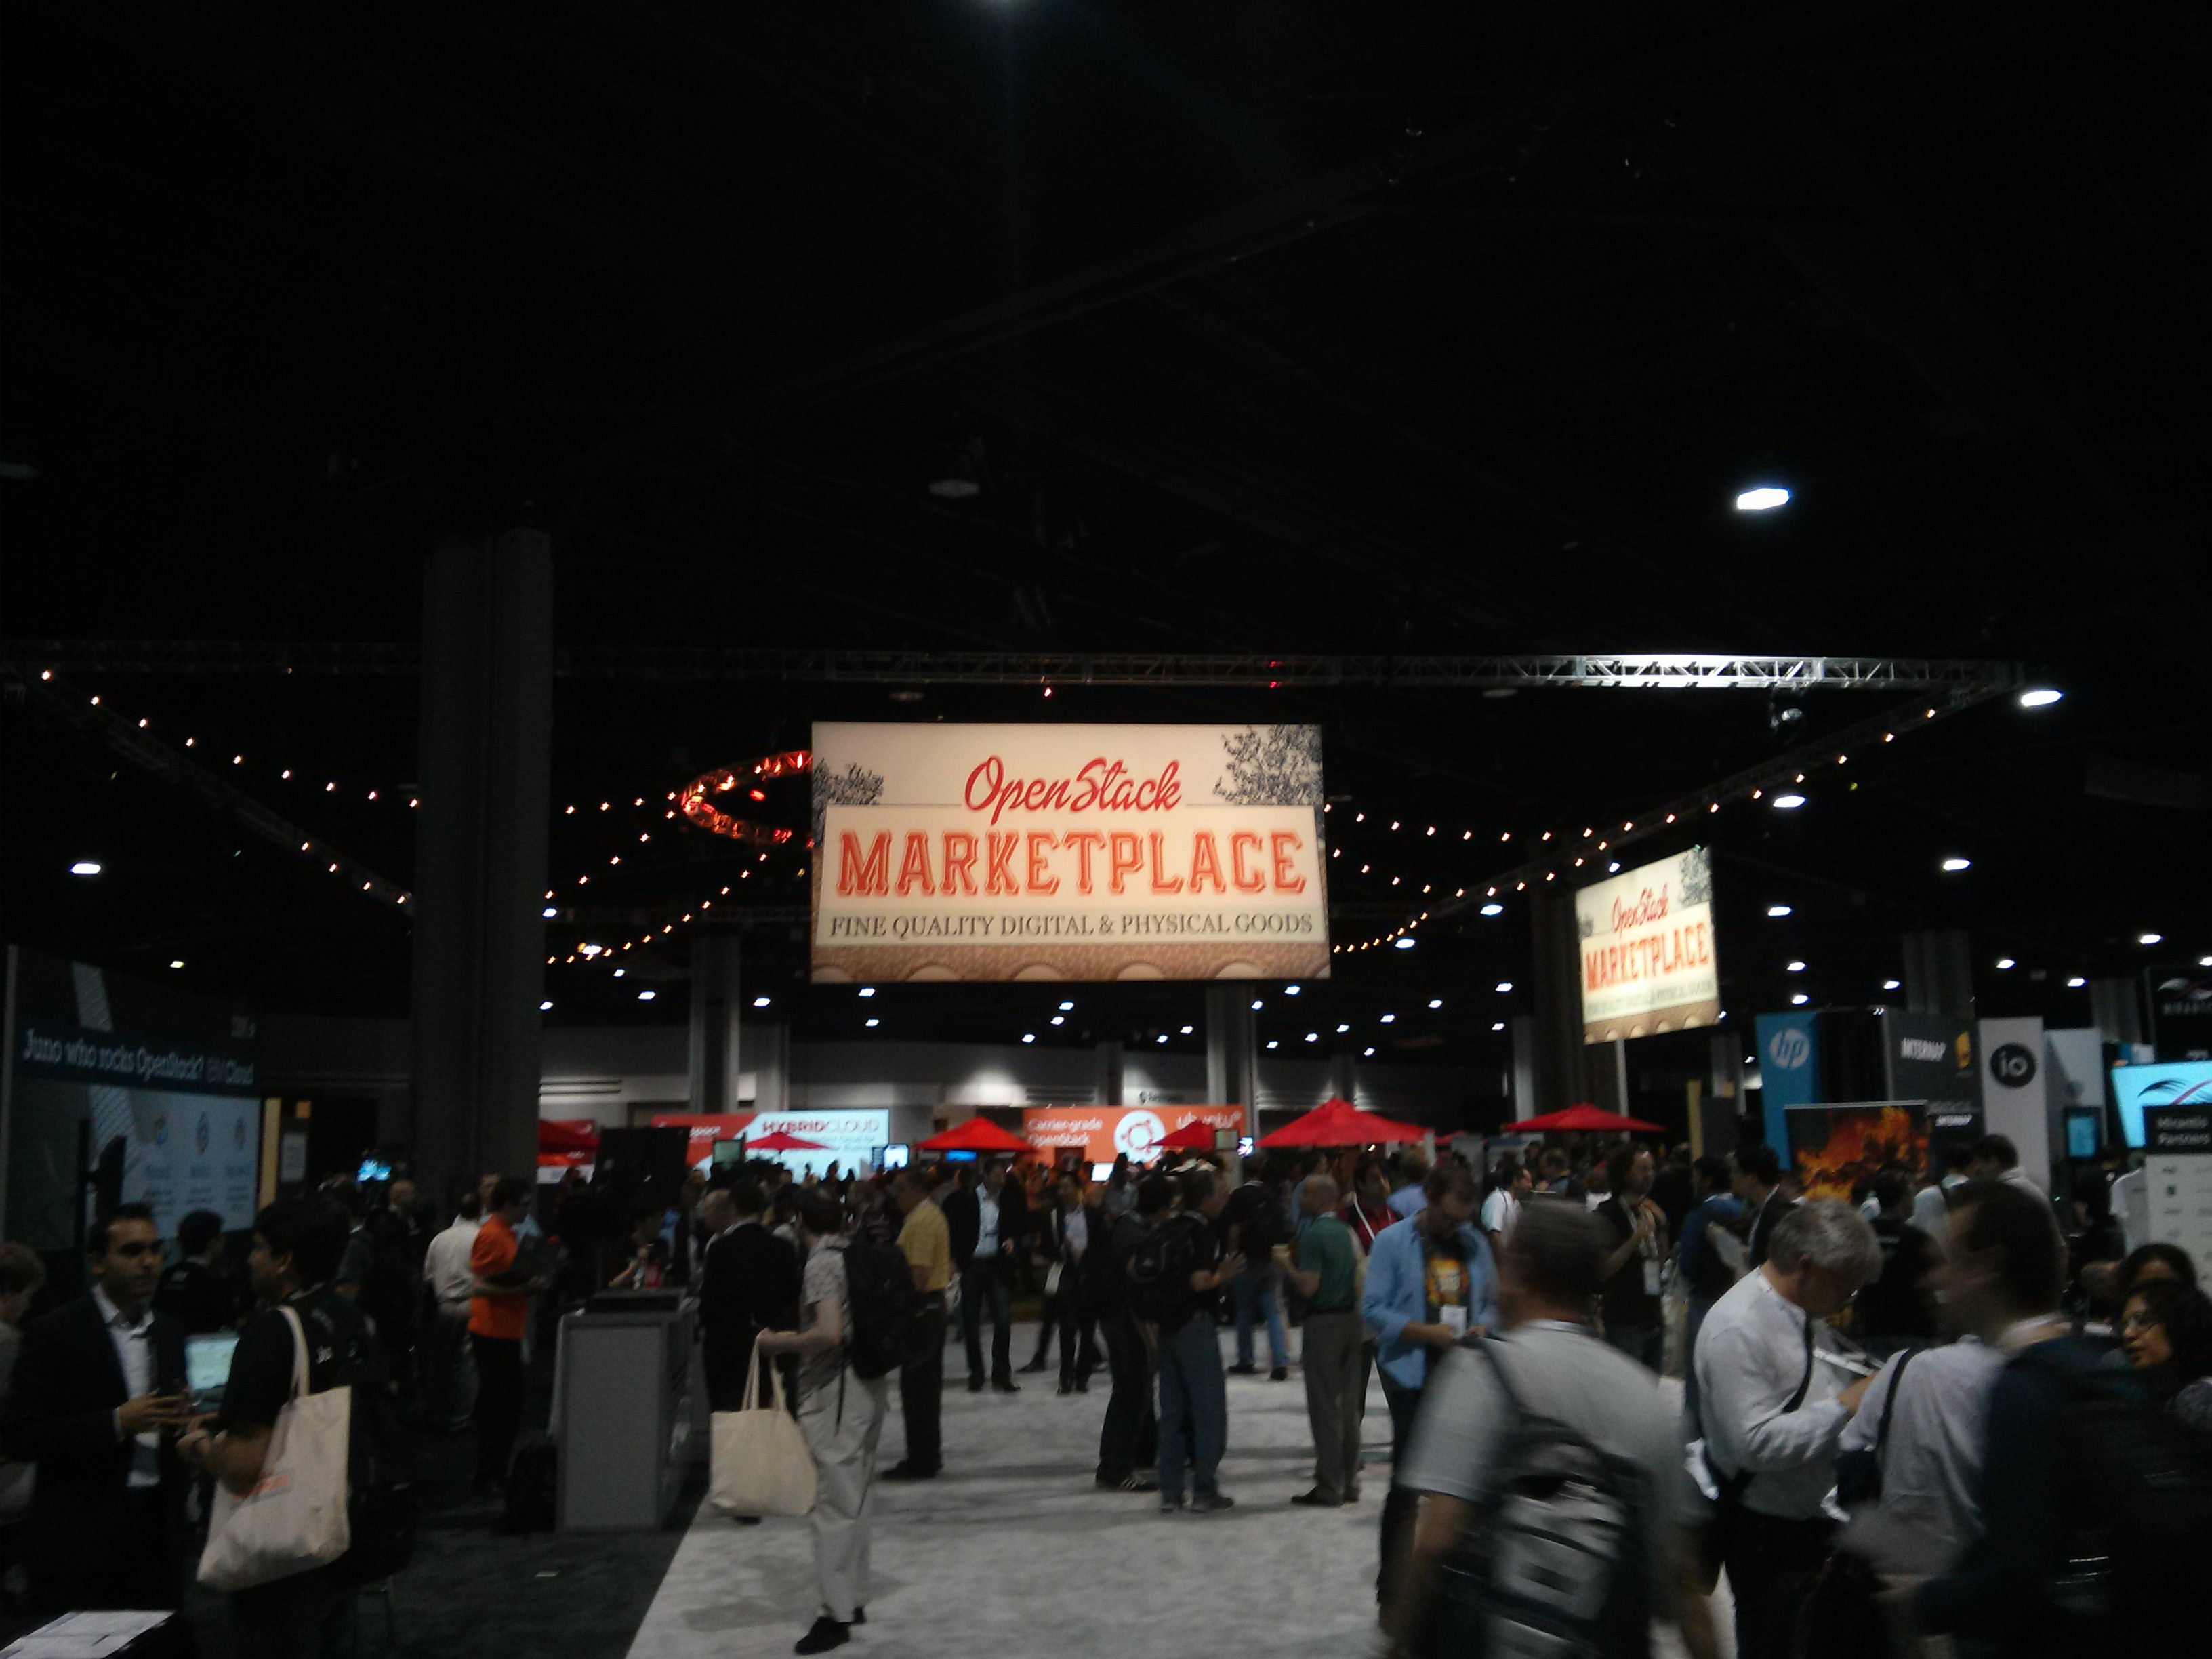
\includegraphics[width=\textwidth]{images/photo-summit2.jpg}
  \end{frame}
  \begin{frame}
    \frametitle{Design Tenets}
    \begin{enumerate}
      \item Scalability and elasticity are our main goals
      \item Any feature that limits our main goals must be optional
      \item Everything should be asynchronous. If you can't do something asynchronously, see \#2
      \item All required components must be horizontally scalable
      \item Always use shared nothing architecture (SN) or sharding. If you can't Share nothing/shard, see \#2
      \item Distribute everything. Especially logic. Move logic to where state naturally exists.
      \item Accept eventual consistency and use it where it is appropriate.
      \item Test everything. We require tests with submitted code. (We will help you if you need it)
    \end{enumerate}
  \end{frame}

  \begin{frame}
    \frametitle{Implémentation}
    \begin{itemize}
      \item Chaque sous-projet est découpé en plusieurs services\pause
      \item Communication entre les services : AMQP (RabbitMQ)\pause
      \item Base de données : relationnelle SQL (MySQL/MariaDB)\pause
      \item Réseau : OpenVSwitch\pause
      \item En général : réutilisation de composants existants\pause
      \item Tout est développé en Python (Django pour la partie web)\pause
      \item APIs supportées : OpenStack et équivalent Amazon\pause
      \item Multi tenancy
    \end{itemize}
  \end{frame}

  \begin{frame}
    \frametitle{Multi-tenant}
    \begin{itemize}
      \item Notion générale : un déploiement du logiciel permet de multiples utilisations
      \item Un cloud OpenStack permet aux utilisateurs de travailler dans des environnements isolés
      \item Les instances, réseaux, images, etc. sont associés à un tenant
      \item Certaines ressources peuvent être partagées entre tenants (exemple : image publique)
      \item On peut aussi parler de "projet"
    \end{itemize}
  \end{frame}

  \begin{frame}
    \frametitle{Architecture}
    \begin{center}
      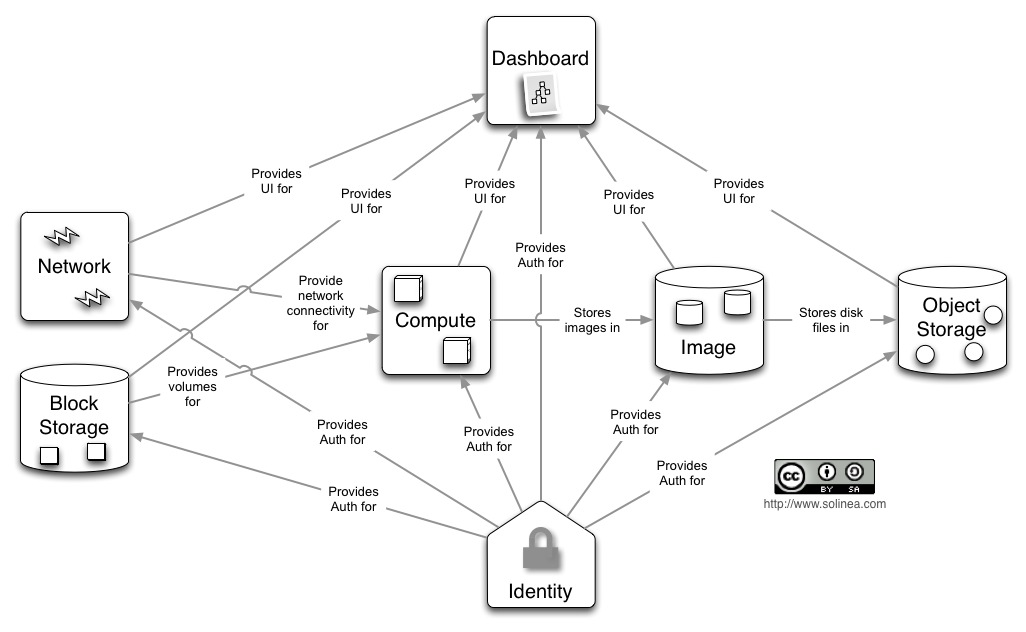
\includegraphics[width=\textwidth]{images/architecture-simple.jpg}
    \end{center}
  \end{frame}

  \begin{frame}
    \frametitle{Interface web / Dashboard : Horizon}
    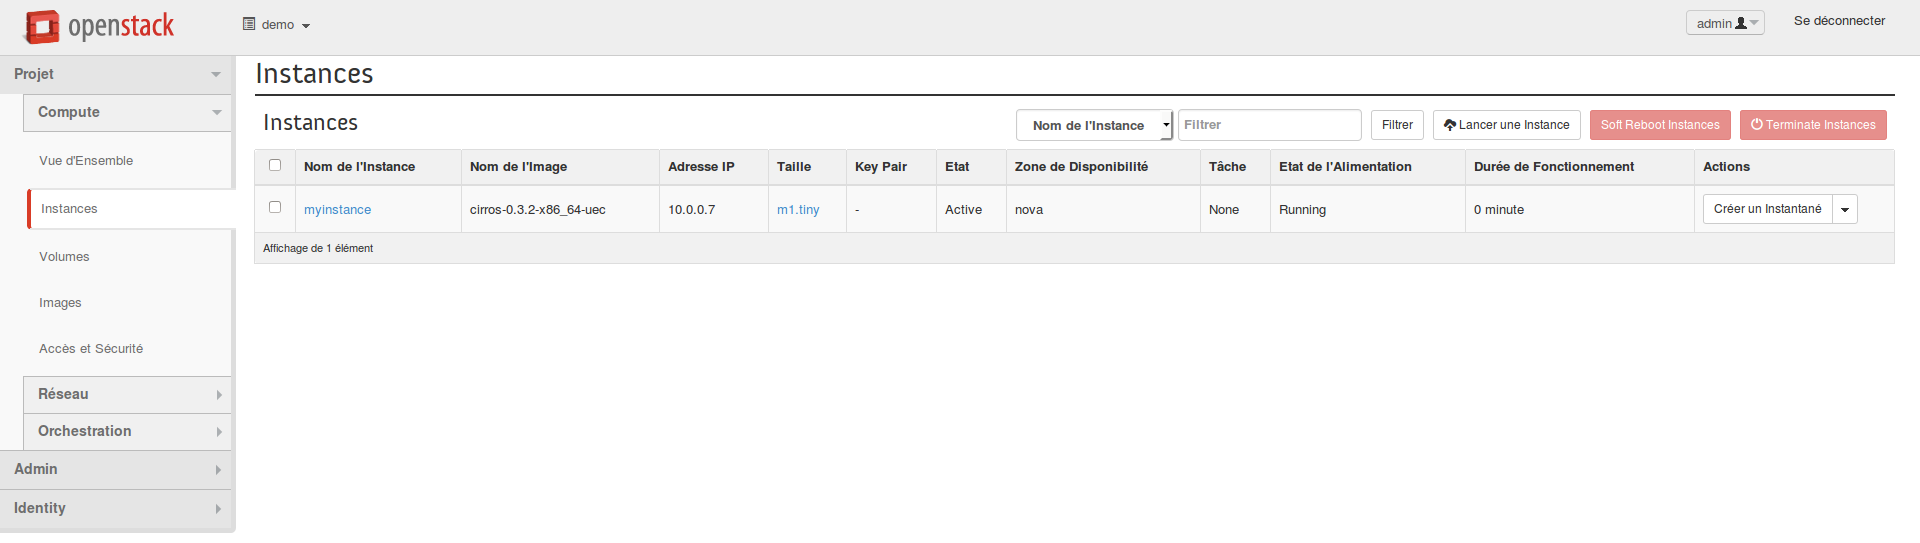
\includegraphics[width=\textwidth]{images/horizon.png}
  \end{frame}

  \begin{frame}
    \frametitle{Ressources}
    \begin{itemize}
      \item Annonces/sécurité : openstack-announce@lists.openstack.org
      \item Documentation : \url{http://docs.openstack.org/}
      \item Support :
      \begin{itemize}
        \item \url{https://ask.openstack.org}
        \item openstack@lists.openstack.org
        \item \#openstack@Freenode
      \end{itemize}
      \item SDK/APIs : \url{http://developer.openstack.org/}
      \item Actualités :
      \begin{itemize}
        \item Blog officiel : \url{http://www.openstack.org/blog/}
        \item Planet : \url{http://planet.openstack.org}
        \item Superuser : \url{http://superuser.openstack.org/}
        \item OpenStack Community Weekly Newsletter
      \end{itemize}
    \item Ressources commerciales : \url{http://www.openstack.org/marketplace/} entre autres
    \end{itemize}
  \end{frame}

  \begin{frame}
    \frametitle{Ressources - Communauté francophone}
    
\includegraphics{images/openstackfr.png}
    \begin{itemize}
      \item Site web : \url{http://openstack.fr/}
      \item Association des utilisateurs francophones d'OpenStack : \url{https://asso.openstack.fr/}
      \item Meetups : Paris, Rhônes-Alpes, Toulouse, Montréal, ...
      \item Présence à des événements tels que Solutions Linux
      \item Canaux de communication :
      \begin{itemize}
        \item openstack-fr@lists.openstack.org
        \item \#openstack-fr@Freenode
      \end{itemize}
    \end{itemize}
  \end{frame}

  \subsection[DevStack]{DevStack : faire tourner rapidement un OpenStack}

  \begin{frame}
    \frametitle{Utilité de DevStack}
    \begin{itemize}
      \item Déployer rapidement un OpenStack
      \item Utilisé par les développeurs pour tester leurs changements
      \item Utilisé pour faire des démonstrations
      \item Utilisé pour tester les APIs sans se préoccuper du déploiement
      \item Ne doit PAS être utilisé pour de la production
    \end{itemize}
  \end{frame}

  \begin{frame}
    \frametitle{Fonctionnement de DevStack}
    \begin{itemize}
      \item Un script shell qui fait tout le travail : stack.sh
      \item Un fichier de configuration : local.conf
      \item Installe toute les dépendances nécessaires (paquets)
      \item Clone les dépôts git (branche master par défaut)
      \item Lance tous les composants dans un screen
    \end{itemize}
  \end{frame}

  \begin{frame}[containsverbatim]
    \frametitle{Configuration : local.conf}
    Exemple
\begin{verbatim}
[[local|localrc]]
ADMIN_PASSWORD=secrete
DATABASE_PASSWORD=$ADMIN_PASSWORD
RABBIT_PASSWORD=$ADMIN_PASSWORD
SERVICE_PASSWORD=$ADMIN_PASSWORD
SERVICE_TOKEN=a682f596-76f3-11e3-b3b2-e716f9080d50
#FIXED_RANGE=172.31.1.0/24
#FLOATING_RANGE=192.168.20.0/25
#HOST_IP=10.3.4.5
\end{verbatim}
  \end{frame}

  \begin{frame}
    \frametitle{Conseils d'utilisation}
    \begin{itemize}
      \item DevStack installe beaucoup de choses sur la machine
      \item Il est recommandé de travailler dans une VM
      \item Pour tester tous les composants OpenStack dans de bonnes conditions, plusieurs Go de RAM sont nécessaires
      \item L'utilisation de Vagrant est conseillée
    \end{itemize}
  \end{frame}

  \subsection[Utilisation]{Utiliser OpenStack}

  \begin{frame}
    \frametitle{Le principe}
    \begin{itemize}
      \item Toutes les fonctionnalités sont accessibles par l'API
      \item Les clients (y compris Horizon) utilisent l'API
      \item Des crédentials sont nécessaires
      \begin{itemize}
        \item API OpenStack : utilisateur + mot de passe + tenant
        \item API AWS : access key ID + secret access key
      \end{itemize}
    \end{itemize}
  \end{frame}

  \begin{frame}
    \frametitle{Accès aux APIs}
    \begin{itemize}
      \item Direct, en HTTP, via des outils comme curl
      \item Avec une bibliothèque
      \begin{itemize}
        \item Les implémentations officielles en Python
        \item D'autres implémentations pour d'autres langages (exemple : jclouds)
      \end{itemize}
      \item Avec les outils officiels en ligne de commande
      \item Avec Horizon
    \end{itemize}
  \end{frame}

  \begin{frame}
    \frametitle{Clients officiels}
    \begin{itemize}
      \item Le projet fournit des clients officiels : python-PROJETclient
      \item Bibliothèques Python
      \item Outils CLI
      \begin{itemize}
        \item L'authentification se fait en passant les credentials par paramètres ou variables d'environnement
        \item L'option --debug affiche la communication HTTP
      \end{itemize}
    \end{itemize}
  \end{frame}
